%\documentclass[a4paper,12pt]{article}
\documentclass[utf8]{bjmc}

\usepackage{amsmath}
\usepackage{graphicx}
\usepackage{amssymb}

\usepackage{tabularx}
\usepackage{makecell}
\usepackage{tcolorbox}
\usepackage{float}
\usepackage{caption}
\usepackage{hyperref}

\pagestyle{empty}
\renewcommand{\thefootnote}{}
%\newtheorem{theorem}{\bf Theorem}
% \newtheorem{lemma}      [theorem] {\bf Lemma}
% \newtheorem{corollary}  [theorem] {\bf Corollary}
% \newtheorem{proposition} [theorem] {\bf Proposition}
% \newtheorem{definition} [theorem] {\bf Definition}
% \newtheorem{remark}     [theorem] {\bf Remark}
% \newtheorem{example}    [theorem] {\bf Example}
% \newtheorem{problem}    [theorem] {\bf Problem}

\setlength{\parindent}{0pt}

\begin{document}


\begin{center}
	 {\bf \large Perfect Polyiamonds: Existence and Properties}
% Mums granta nav :(
%	\footnote{{\bf Acknowledgement}  The support of the grant ...... is kindly announced.}
\end{center}

\vspace{0.1cm}

% \begin{center}\large {
% APSĪTIS Kalvis$^1$
% \  and  \
% RUDZĀTE Marta$^1$}
% \end{center}
% \begin{center}
% \it {
% $^1$ University of Latvia, 
% Raiņa bulvāris 19, 
% Latvia \\
% E-mail: {\rm kalvis.apsitis@gmail.com} \\
% \vspace{1mm}
% E-mail: {\rm martarudzate@gmail.com }}
% \end{center}
% \vspace{0.2cm}

\begin{abstract}
Perfect polyiamonds are a subclass of polyiamonds where the 
$n$ sides take all lengths from $1$ to $n$. 
In this article perfect polyiamonds illustrate how 
the concepts formal languages and string manipulation algorithms 
become combinatiorial geometry examples. 
\end{abstract}

\section{Introduction}


\begin{definition}
A {\em polyiamond} is a simple polygon made of equilateral triangles. A {\em perfect $n$-polyiamond}\cite{APSITIS1} 
is a polyiamond whose sides are of lengths $n,n-1,\ldots,1$ in this order. 
A {\em perfect acute polyiamond} has all interior angles $60^{\circ}$ or $300^{\circ}$, 
a {\em perfect obtuse polyiamond} has all interior angles $120^{\circ}$ or $240^{\circ}$.
\end{definition}

Perfect polyiamonds can be represented as strings over the alphabet 
$\Sigma = \{ \mathtt{a}, \mathtt{b}, \mathtt{c}, \mathtt{d}, \mathtt{e}, \mathtt{f} \}$
listing their side directions in decreasing length order. 



{\centering{
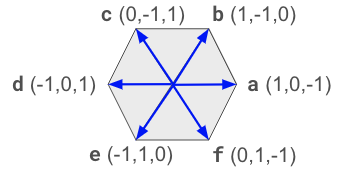
\includegraphics[width=2.5in]{direction-vectors.png}
\captionof{figure}{Coordinates for direction vectors on a triangular grid}
\label{fig:coord_2}
}} 



To avoid analyzing polyiamonds that only differ by rotation and axial symmetry, 
we typically assume that the first (the longest) side goes in the direction $\mathtt{a}$
(to the east), and the second longest side goes either in direction $\mathtt{b}$
(to the north-east) or in direction $\mathtt{c}$ (to the north-west). 


In this article we show the existence of perfect (also perfect acute, perfect obtuse)
polyiamonds for any sufficiently large $n$, except those $n$, where 
simple invariants prevent their existence. 



{\small
\begin{table}[H]
\centering
\caption{The Count of Perfect Polyiamonds by Number of Sides}\label{tab:tab1}
\setlength{\tabcolsep}{5.1pt}

\begin{tabular}{!{\vrule width 1.5pt}l!{\vrule width 1.5pt}c|c|c|c|c|c|c|c|c|c|c|c|c|c!{\vrule width 1.5pt}}
\Xhline{1.5pt}
$\mathbf{n}$ & $5$ & $6$ & $7$ & $8$ & $9$ & $10$ & $11$ & $12$ & $13$ & $14$ & $15$ & $16$ & $17$ & $18$ \\ \hline
\textbf{Count} & $1$ & $1$ & $2$ & $7$ & $3$ & $4$ & $21$ & $87$ & $228$ & $477$ & $1335$ & $4026$ & $8599$ & $22326$ \\ 
\Xhline{1.5pt}
\end{tabular}

\vspace{2mm}

\begin{tabular}{!{\vrule width 1.5pt}l!{\vrule width 1.5pt}c|c|c|c|c|c|c|c!{\vrule width 1.5pt}}
\Xhline{1.5pt}
$\mathbf{n}$ & $19$ & $20$ & $21$ & $22$ & $23$ & $24$ & $25$ & $26$ \\ \hline
\textbf{Count} & $67068$ & $193445$ & $526694$ & $1464978$ & $4284617$ & $12621026$ & $35662687$ & $102848450$ \\ 
\Xhline{1.5pt}
\end{tabular}
\end{table}
}

Even though there is a large number of polyiamonds for large $n$, there is no trivial proof that there is at least one 
perfect polyiamond for each $n \geq 5$. 
This article shows how to build sequences of perfect polyiamonds to cover all sufficiently large $n$ and 
to answer all the existence questions for perfect polyiamonds (as well as both sequential isogon families of perfect polyiamonds).
Apart from existence results, the methods covered here show how to get estimates for area and other properties of perfect polyiamonds
that are close to the theoretical minimum or maximum.
The polyiamond sequences are being generated by formal languages (such as Context-Free Grammars 
or Parallel Context-Free Grammars); so there are families of geometric shapes to illustrate 
non-trivial formal languages. 



\section{Necessary Conditions for Perfect Polyiamonds}

As we noted in the introduction, each perfect polyiamond can be represented as a string over the direction alphabet 
$\Sigma = \{ \mathtt{a}, \mathtt{b}, \mathtt{c}, \mathtt{d}, \mathtt{e}, \mathtt{f} \}$. 
Clearly, not all strings correspond to perfect polyiamonds, as the polygonal chain defined by the string
may not return to the origin, or it may have self-intersections. We discuss these conditions separately. 

\subsection{The Return to Origin Condition}


For a perfect $n$-polyiamond to exist, the sum of the direction vectors must be $(0,0,0)$. 
This condition is easy to check for an individual polygonal chain, but for a family of polygonal chains we 
will use linear algebra conditions. 

In 2024, at a
\href{https://conferences.lu.lv/event/493/contributions/2217/}{discrete
mathematics conference}, the presentation ``Families of Perfect Polyiamonds
and Formal Languages" had a claim and a theorem to show which constructions 
return to the starting point, if the construction is defined by a string expression 
equivalent to a parallel context-free grammar. 

Throughout what follows, we will use the coordinate system shown in
Figure~\ref{fig:coord_2}.

\begin{claim}\label{ap:1}

Given $k$ vectors $u_1,  \dots, u_k$ and $k$ second-degree polynomials
$P_i(t)$. We define
\[
v_n=\sum_{i=1}^k P_i(n)\cdot u_i.
\]
Then all $v_4, v_5, \dots $\ are linear combinations of $v_1, v_2, v_3$.
\end{claim}



\begin{proof}
For each $n$, we define the coefficients
\[
\alpha(n)=\frac{(n-2)(n-3)}{2}, \qquad
\beta(n)=-(n-1)(n-3), \qquad
\gamma(n)=\frac{(n-1)(n-2)}{2}.
\]

Then $
v_n=\alpha(n)v_1+\beta(n)v_2+\gamma(n)v_3,
$
because both sides are identical second-degree polynomials in $n$ with equal
values at the points $n=1,2,3$, and a second-degree polynomial that coincides
at three points is uniquely determined.

\end{proof}


\begin{theorem}\label{th:1}
If \   $s_n =
x_k y_k^{n} x_{k-1} y_{k-1}^{n} \cdots
x_2 y_2^{n} x_1 y_1^{n} x_0
$ \
is a perfect closed polygonal chain, where
$
n = 1,2,3,
$
then the direction sequence $s_n$ describes a perfect polyiamond
(or at least a perfect closed polygonal chain that returns to the starting
point) for all natural numbers $n$.
\end{theorem}
\begin{proof}


For any string of letters
$x=\mathtt{x}_1\ldots{}\mathtt{x}_L$ of length $L = |x|$, we define
the following two functions whose values are vectors in our triangular-grid
coordinate system $\mathbb{Z}^3$:
\[
\begin{array}{rcl}
g(x) & = & \sum_{j = 1}^{L} (L - j + 1) \cdot \mathbf{h}(\mathtt{x}_j),\\
p(x) & = & \sum_{j = 1}^{L} \mathbf{h}(\mathtt{x}_j),\\
\end{array}
\]
where $\mathbf{h}(\mathtt{x}_j)$ denotes the unit vector corresponding to the
$j$-th direction letter in the string $x$:
$\mathtt{x}_j \in \{ \mathtt{a}, \mathtt{b}, \mathtt{c}, \mathtt{d},
\mathtt{e}, \mathtt{f}\}$. These unit vectors are, respectively,
$\mathbf{h}(\mathtt{a}) = (1,0,-1)$,
$\mathbf{h}(\mathtt{b}) = (1,-1,0)$,
$\mathbf{h}(\mathtt{c}) = (0,-1,1)$,
$\mathbf{h}(\mathtt{d}) = (-1,0,1)$,
$\mathbf{h}(\mathtt{e}) = (-1,1,0)$,
$\mathbf{h}(\mathtt{f}) = (0,1,-1)$.


The sum of the edge vectors for arbitrary $n$:
\[
v_n =
g(x_0)
+
\sum_{i=1}^{k}
\bigl(g(y_i)+g(x_i)\bigr)+
\]
\[
+
\sum_{i=1}^{k}
\left(
n\cdot |x_0|
+
\sum_{j=1}^{i-1}
n\cdot (n\cdot |y_j| + |x_j|)
+
\frac{n(n-1)}{2}|y_i|
\right)
\cdot v(y_i)+
\]
\[
+
\sum_{i=1}^{k}
\left(
|x_0|
+
\sum_{j=1}^{i-1}
(n\cdot |y_j| + |x_j|)
+
n\cdot |y_i|
\right)
\cdot v(x_i).
\]



\bigskip

All the remaining vectors can be expressed in terms of the vectors
$v_1,v_2,v_3$ -- see Claim \ref{ap:1} above.
If $v_1,v_2,v_3=(0,0,0)$,
then also $v_4, v_5, ... =(0,0,0)$, i.e.\ all closed polygonal chains will return
to the starting point.

\end{proof}



\subsection{The Non-Intersection Condition}

We do not have a general theory for the non-intersection condition for any sequence $w_k \in \Sigma^{\ast}$ of 
perfect polygonal chains returning to the origin. The reason why general theory may be complicated is 
that there are counterexamples -- perfect polygonal chains returning to the origin and having 
some initial members that are perfect polyiamonds, but for some larger values of $k$ the sides intersect.
They may intersect for all sufficiently large $k$, or just for some sporadic values of $k$. 


% NEW_n8_125,a (cb)^k cd (fe)^k fd (ea)^k fbf (de)^k,8,8,4

\begin{example}
Consider perfect polygonal chains defined for all $n = 8k + 8$ by the following string expresison: 
$E^{(8,8,Inter1)} = \mathtt{a} (\mathtt{cb})^k \mathtt{cd} (\mathtt{fe})^k \mathtt{fd} (\mathtt{ea})^k \mathtt{fbf} (\mathtt{de})^k$. 
\end{example}

The first three polyiamonds in this sequence satisfy Theorem~\ref{th:1}; so all polygonal chains in this sequence return to the origin, 
and for $k=0,1,2,3,4$ they are perfect polyiamonds. Nevertheless, the sides intersect for $k \geq 5$.


{\centering{
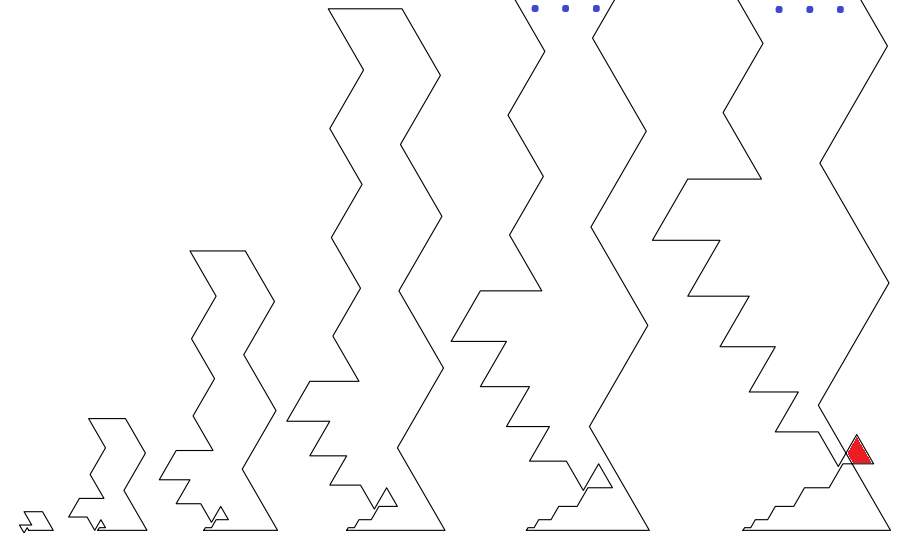
\includegraphics[width=4.5in]{self_intersect_1.png}
\captionof{figure}{Polyiamond sequence with self-intersections for all $k \geq 5$.}
\label{fig:self_intersect_1}
}} 






\begin{example}
Consider perfect polygonal chains defined for all $n = 8k + 11$ by the following string expresison: 
$(\mathtt{ac})^k \mathtt{abdfdb} (\mathtt{df})^k \mathtt{de} (\mathtt{fd})^k \mathtt{fdf} (\mathtt{ac})^k$. 
For $k=0,1,2,3,4$ the polygonal chains are perfect polyiamonds, but for $k=5$ the sides intersect.
({\em Note: } Intersections occur for larger $k$ as well -- in particular for $k=17$, $k=35$, $k=59$, and $k=89$).
\end{example}

{\centering{
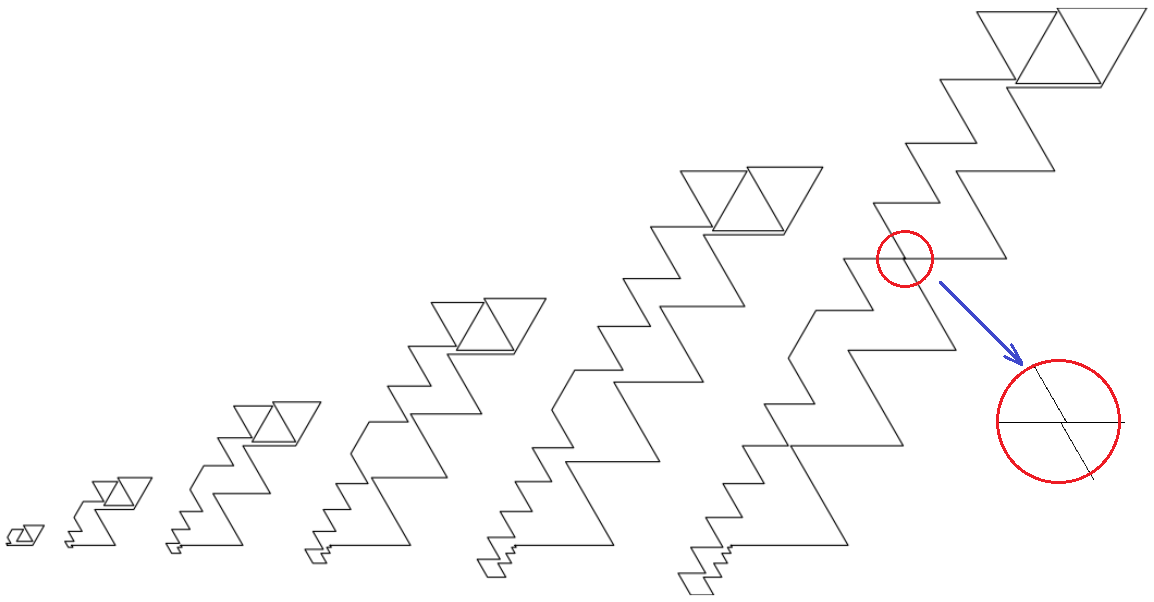
\includegraphics[width=4.5in]{self_intersect_2.png}
\captionof{figure}{Polyiamond sequence with self-intersections for a few values of $k$.}
\label{fig:self_intersect_2}
}} 




Fortunately, for existence of perfect polynomials we can choose string expressions that are convenient 
for non-intersection proofs, where the zigzags of the sides are separated and cannot intersect. 




% WARNING: NEW_n11_392: the side sequence for k=5 intersects itself
% WARNING: NEW_n11_392: the side sequence for k=17 intersects itself
% WARNING: NEW_n11_392: the side sequence for k=35 intersects itself
% WARNING: NEW_n11_392: the side sequence for k=59 intersects itself
% WARNING: NEW_n11_392: the side sequence for k=89 intersects itself



\section{The Existence of Perfect Polyiamonds}

This section states the necessary and sufficient conditions for 
having an $n$-sided perfect polyiamond as well as its subfamilies
(serial $60^{\circ}$ and serial $120^{\circ}$ isogons).

\begin{theorem}
For any integer $n \geq 5$ there exists a perfect $n$-polyiamond.
\end{theorem}


% NEW_n5_3,ac (bdfd)^k edf (afab)^k,5,8,2
% NEW_n6_9,a (bd)^k ce (df)^k d (fa)^k f (ba)^k b,6,8,4
% NEW_n7_18,a (cb)^k cd (fe)^k (df)^k e (fa)^k fbf,7,8,4


\begin{proof}

Consider the following string expressions: 

\[
\begin{array}{ccl}
E^{(8,5)}_k & = & \mathtt{ac}(\mathtt{bdfd})^k\,\mathtt{edf}(\mathtt{afab})^k \\
E^{(8,6)}_k & = & \mathtt{a}(\mathtt{bd})^k\,\mathtt{ce}(\mathtt{df})^k\,\mathtt{d}(\mathtt{fa})^k\,\mathtt{f}(\mathtt{ba})^k\,\mathtt{b} \\
E^{(8,7)}_k & = & \mathtt{a}(\mathtt{cb})^k\,\mathtt{cd}(\mathtt{fe})^k\,\mathtt{(df)}^k\,\mathtt{e}(\mathtt{fa})^k\,\mathtt{fbf} \\
E^{(8,8)}_k & = & \mathtt{ab}(\mathtt{ab})^k\,\mathtt{dede}(\mathtt{dede})^k\,\mathtt{ab}(\mathtt{ab})^k \\
E^{(8,9)}_k & = & \ldots \\
E^{(8,10)}_k & = & \ldots \\
E^{(8,11)}_k & = & \ldots \\
E^{(8,12)}_k & = & \ldots \\
\end{array}
\]

TBD. Need to prove that the expressions generate perfect polygonal chains that do not self-intersect. 
\end{proof}

\subsection{The Existence of Perfect Acute Polyiamonds (Serial $60^{\circ}$ Isogons)}


\begin{theorem}
For a perfect acute $n$ polyiamond to exist, we must have $n \equiv 3 \pmod 6$ or $n \equiv 5 \pmod 6$. 
\end{theorem}

\begin{proof}
{\bf (1) $n$ must be odd.} Let $m$ denote the number of $60^{\circ}$ angles, 
and $(n-m)$ is the number of $300^{\circ}$ angles. The sum of internal angles: 
\[ (n-2) \cdot 180^\circ = m \cdot 60^\circ + (n-m) \cdot 300^\circ \]
After simplification we get $4m = 2n + 6$ or $n = 2m - 3$, so $n$ is odd.

{\bf (2) $n$ cannot be $\equiv 1 \pmod 3$.} 
Side directions in an acute polyiamond are $\mathtt{a}$, $\mathtt{c}$ or $\mathtt{e}$. 
For the three directions to cancel each other out, the number of sides in each direction must be the same.
Thus, $n(n+1)/2$ must be divisible by $3$, which cannot happen if $n \equiv 1 \pmod 3$.

Combining (1) and (2) we get  $n \equiv 3 \pmod 6$ or $n \equiv 5 \pmod 6$
\end{proof}

\begin{theorem}
Perfect acute $n$-polyiamonds exist for $n=9$ and all $n \geq 27$ such that $n \equiv 3 \pmod 6$ or $n \equiv 5 \pmod 6$.
\end{theorem}

\begin{proof}
TBD. (Need to build acute polyiamond sequences to cover all viable $n$.)
\end{proof}




\subsection{The Existence of Perfect Obtuse Polyiamonds (Serial $120^{\circ}$ Isogons)}


\begin{theorem}
For a perfect obtuse $n$ polyiamond to exist, it is necessary 
to have $n \equiv 0 \pmod 6$. 
\end{theorem}

\begin{proof}
{\bf (1) $n$ must be even.} 
By contradiction, assume that $n = 2k + 1$. Then the sum of internal angles is
$180^{\circ}(2k-1)$. Each internal angle 
is either $120^{\circ}$ or $240^{\circ}$; let $m$ denote the number of $120^{\circ}$
angles. Then

\begin{align}
(2k-1) \cdot 180^{\circ} & = m \cdot 120^{\circ} + (2k-1-m) \cdot 240^{\circ}, \nonumber \\
3(2k-1) & = 2m + 4(2k-1-m), \nonumber \\
2m - 3 & = 2k - 4. \nonumber \\ 
\end{align}
This is a contradiction: $1 \equiv 0 \pmod 2$. 

{\bf (2) $n$ must be divisible by $3$.}
Assume that your polyiamond starts in a triangle grid point with coordinates
$(0,0,0)$. From (1) we know that $n = 2k$ is even, so the first side in the direction 
$\mathtt{a}$ is of even length $2k$. 
After side $\mathtt{a}$, the next side can be in either 
$\mathtt{b}$ or $\mathtt{f}$ to have an obtuse angle with the previous side. 

Because of parity invariant we conclude that all sides of even 
length are in directions $\mathtt{a,c,e}$ (red vectors), 
and all sides of odd length are in directions $\mathtt{b,d,f}$ (blue vectors).

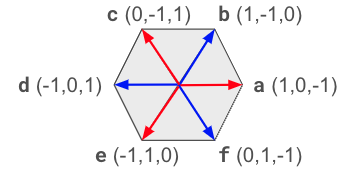
\includegraphics[width=2.5in]{colored-direction-vectors.png}

Denote the vertices of the $n$-polyiamond by $P_0 = (0,0,0)$, 
$P_1 = (x_1,y_1, z_1)$, $P_2 = (x_2,y_2,z_2)$, $\ldots$, 
$P_{2k-1} = (x_{2k-1},y_{2k-1},z_{2k-1})$, $P_{2k} = (0,0,0)$
(after traversing all $n=2k$ vectors it must return back to the origin).

Observe that adding a red vector (of even length) the difference $(x_i - y_i)$ 
will change to $(x_{i+1} - y_{i+1})$ -- and the difference 
$$(x_{i+1} - y_{i+1}) - (x_i - y_i) \equiv 2 \pmod 3,$$
since for each red vector $\mathtt{a,c,e}$ the difference between $x$ and $y$ is 
either $1-0$, $0-(-1)$, or $(-1) - 1$. All these numbers are $\equiv 1 \pmod 3$
or $\equiv 2 \pmod 3$ after being multiplied by an even number (the side length) 

Similarly, adding a blue vector (of odd length), the difference 
$$(x_{i+1} - y_{i+1}) - (x_i - y_i) \equiv 2 \pmod 3,$$
since for each blue vector $\mathtt{a,c,e}$ the difference between $x$ and $y$ is 
either $1-(-1)$, $(-1)-0$, or $0 - 1$. All these numbers are $\equiv 2 \pmod 3$
and they will stay $\equiv 2 \pmod 3$ after being multiplied by an 
odd number (the side length). 

So, after adding each side (red or blue), the difference 
$(x_{i+1} - y_{i+1}) - (x_i - y_i)$ changes by $2$ (modulo $3$). 
Since it has to return back to $(0,0,0)$, we conclude that the number of 
sides must be divisible by $3$. 

Combining (1) and (2) we get  $n \equiv 0 \pmod 6$
\end{proof}


{\em Note:} See also the 
{\em Baltic Way 2025} -- the solution of Problem 9. 


In \cite{Sallows1991} it is stated that ``serial 120-degree isogons exist if and only if $n$ is divisible by $6$''. 
This is almost true (as they do not exist for $n = 6$). We have the following refinement:

\begin{theorem}
For any integer $n \geq 12$ divisible by $6$ there exists an obtuse perfect 
$n$-polyiamond.
\end{theorem}

\begin{proof}
There are two expressions that generate sequences of perfect polyiamonds with side counts 
$12, 24, 36,\ldots$ and
$18, 30, 42, \ldots$ respectively. 


Consider the following expression: 
\[
E^{(12,12)}_k = (\mathtt{ab})^k\mathtt{abc}(\mathtt{de})^k\mathtt{de}(\mathtt{dc})^k\mathtt{de}(\mathtt{fa})^k\mathtt{fa}(\mathtt{fe})^k\mathtt{fa}(\mathtt{bc})^k\mathtt{b}
\]


{\centering{
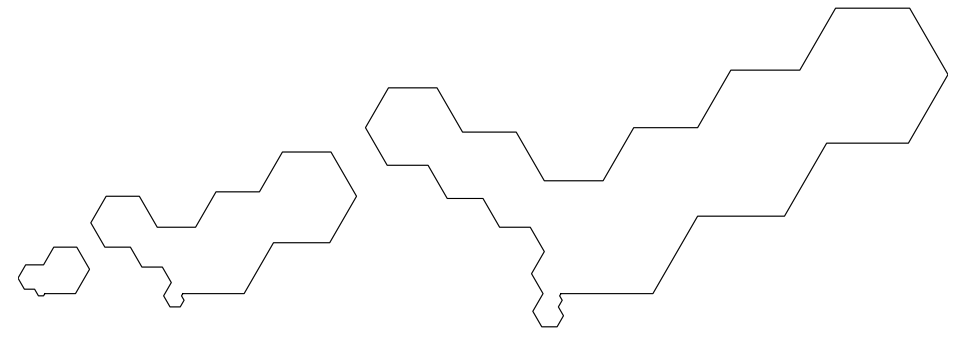
\includegraphics[width=3.5in]{120isogon_12_24_36.png}
\captionof{figure}{Polygons in the sequence $E^{(12,12)}_k$ for $k=0,1,2$.}
\label{fig:120isogon_12_24_36}
}} 

And also the second expression: 

\[
E^{(12,18)}_k = (\mathtt{ab})^k\mathtt{abaf}(\mathtt{ed})^k\mathtt{eded}(\mathtt{ef})^k\mathtt{ed}(\mathtt{cb})^k\mathtt{cbcb}(\mathtt{cd})^k\mathtt{cb}(\mathtt{af})^k\mathtt{ab},\;\;\;\mbox{kur $k = 0,1,2,\ldots$}
\]


{\centering{
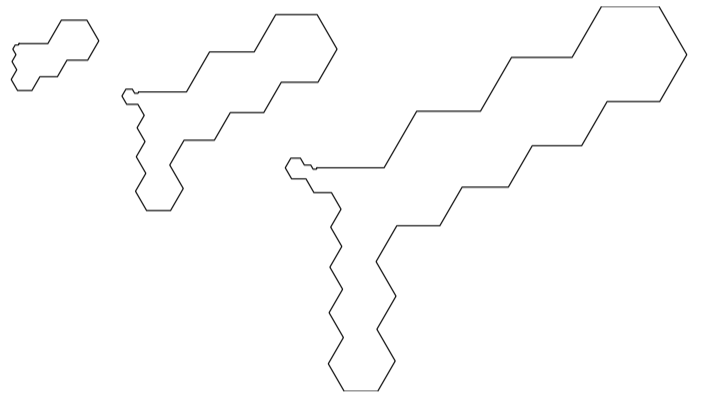
\includegraphics[width=3.5in]{120isogon_18_30_42.png}
\captionof{figure}{Polygons in the sequence $E^{(12,18)}_k$ for $k=0,1,2$.}
\label{fig:120isogon_18_30_42}
}} 



If we check the adjacent letters in both sequences, we notice that the letters 
$\mathtt{a} \leftrightarrow \mathtt{b}  \leftrightarrow \mathtt{c}  \leftrightarrow \mathtt{d}  \leftrightarrow \mathtt{e}  \leftrightarrow \mathtt{f}  \leftrightarrow \mathtt{a}$
are the only possible pairs of neighboring letters. Since their directions differ by $60^{\circ}$, 
any two adjacent sides in the polyiamond make a $120^{\circ}$ (or a $240^{\circ}$) angle. 
In both expressions, the first three members ($k=0,1,2$) return to the origin, 
so they satisfy the condition of Theorem~\ref{th:1}, and all the subsequent members will also be closed polygonal chains. 


Regarding non-intersection, the zigzags of the sides are separated. 

{\centering{
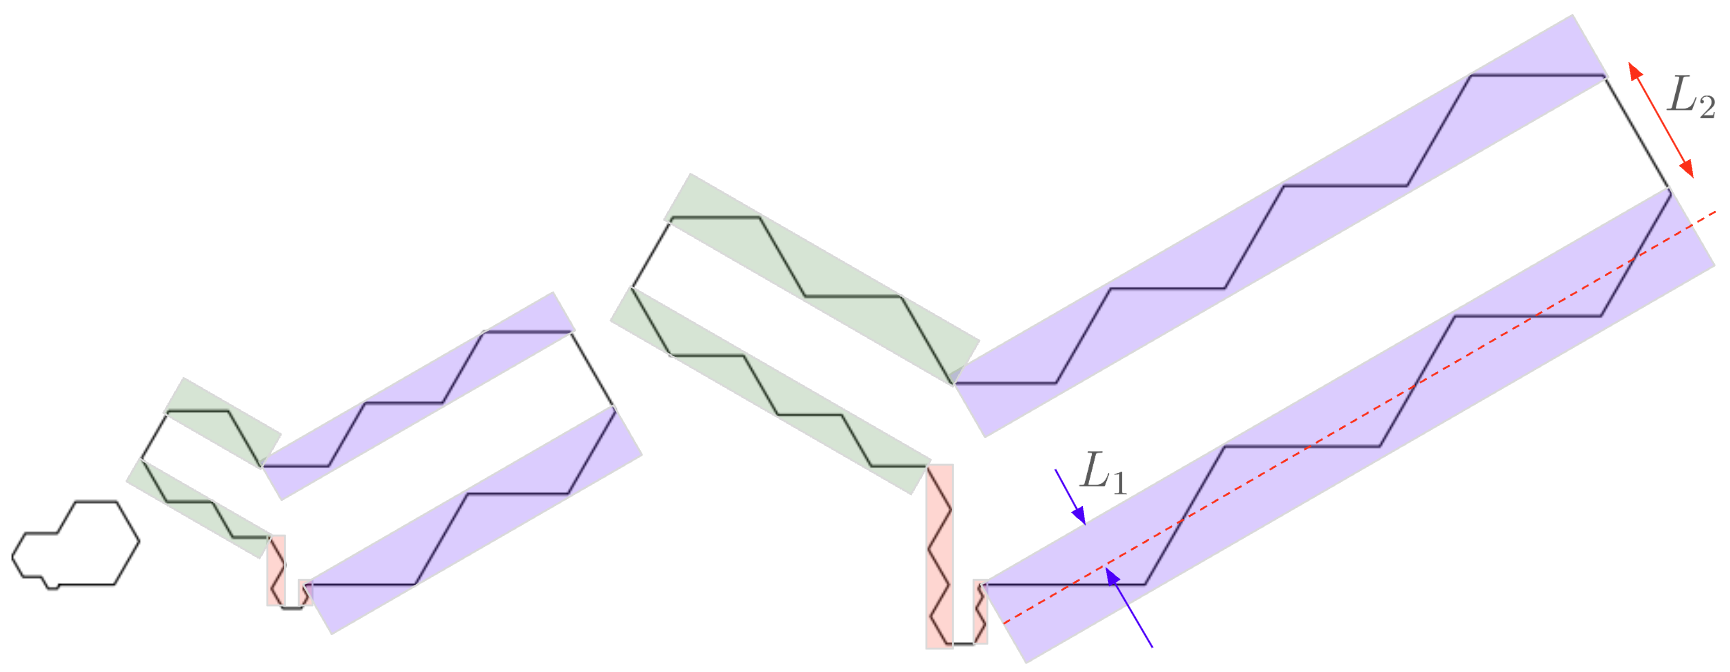
\includegraphics[width=3.5in]{120-isogon-non-intersection.png}
\captionof{figure}{The separation between sides in $E^{(12,12)}_k$.}
\label{fig:120-isogon-non-intersection}
}} 
\end{proof}








\section{The Existence of Magic Polyiamonds}

In this section we relax the requirements on the perfect polyiamonds by allowing any permutation of the sides. 

\begin{definition}
A {\em magic $n$-polyiamond} is a polyiamond with $n$ sides of pairwise different lengths 
taking values in $\{ 1,\ldots n\}$. 
\end{definition}

Magic polyiamonds are a generalization of perfect ones. To define a 
magic polyiamond we need to know
the direction vectors for all sides, and additionally the permutation 
of the side lengths. 


\begin{theorem}[Given permutation, pick directions]
For any $n \geq 9$ and any permutation 
of the numbers $[1;n]$ there exists a 
magic polyiamond with side lengths corresponding to that permutation. 
\end{theorem}

TBD.


\begin{theorem}[Given directions, pick permutation]
For any sufficiently large $n$, and each set of 
$n$ direction vectors $\mathbf{v}_1, \mathbf{v}_2, \ldots, \mathbf{v}_n$
such that no more than half is in the same pair of directions 
$(\mathtt{a}, \mathtt{d})$, $(\mathtt{b}, \mathtt{e})$, $(\mathtt{c}, \mathtt{e})$, 
and their sum is $(0,0,0)$, one can rearrange these vectors so that 
they make a magic polyiamond (without intersecting or overlapping sides).
\end{theorem}

TBD.



\section{Areas of Perfect Polyiamonds}

\begin{theorem}[Finite Difference Theorem]
Let $f:\mathbb{N}_{\geq n_0}\to \mathbb{R}\) be a function on all positive integers $n \geq n_0$. Define the \emph{forward difference} operator \(\Delta\):
\[
(\Delta f)(n)=f(n+1)-f(n),
\]
and define higher differences recursively by
$\Delta^0 f=f$, and $\Delta^{k+1}f=\Delta(\Delta^k f)$.

Then $f(n)$ equals a polynomial $P(n)$ of degree at most $d$ if and only if 
there is a constant $C$ such that
$\Delta^{d}f(n)=C$ for all $n\geq n_0$.
\end{theorem}


\begin{theorem}
For any sequence of perfect polyiamonds generated by a string expression of the form
\[E(k) = x_m y_m^{n} x_{m-1} y_{m-1}^{n} \cdots x_2 y_2^{n} x_1 y_1^{n} x_0 \]
the area sequence $A(\mathcal{P}_k)$ is a polynomial in $k$ of degree either $3$ or $4$.
\end{theorem}

\begin{proof}
TBD.
Proof uses the finite difference theorem and express the area of any perfect polyiamond through
the formula of determinants of the vertex coordinates (the shoelace formula). 
If all the inserted strings $y_i$ have their corresponding unit vector sums collinear, then it is a polynomial of degree $3$, 
otherwise it is a polynomial of degree $4$.
\end{proof}

\begin{example}
Consider the expression $E^{(8,5)}_k = \mathtt{ac}(\mathtt{bdfd})^k\,\mathtt{edf}(\mathtt{afab})^k$ 
generating perfect polyiamonds $\mathcal{P}^{(8,5)}_0, \mathcal{P}^{(8,5)}_1, \mathcal{P}^{(8,5)}_2, \ldots$ 
with side counts $n = 5, 13, 21, \ldots$ ($n = 8k + 5$ in general). 
The area of these polyiamonds is a polynomial in $k$ of degree $3$: 
\[ A(\mathcal{P}^{(8,5)}_k) = 144k^3 + 232k^2 + 124k + 19 \]
\end{example}


{\centering{
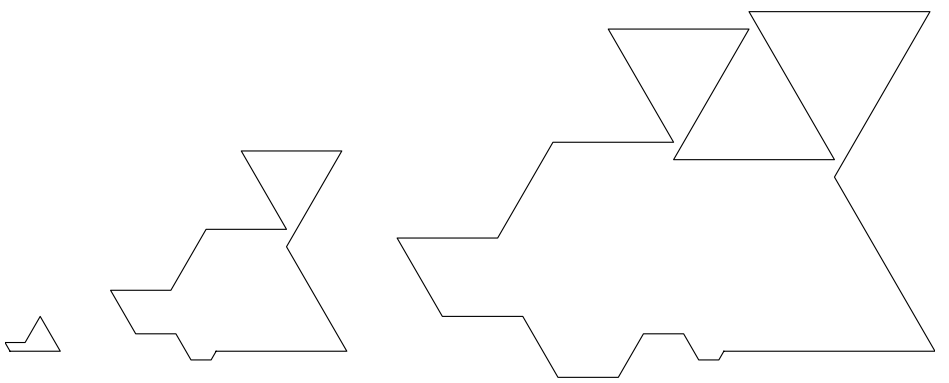
\includegraphics[width=3.5in]{3rd_degree_area.png}
\captionof{figure}{Polyiamond sequence $\mathcal{P}^{(8,5)}_k$.}
\label{fig:3rd_degree_area}
}} 


\begin{example}
Consider the expression $E^{(8,6)}_k = \mathtt{a}(\mathtt{bd})^k\,\mathtt{ce}(\mathtt{df})^k\,\mathtt{d}(\mathtt{fa})^k\,\mathtt{f}(\mathtt{ba})^k\,\mathtt{b}$ 
generating perfect polyiamonds $\mathcal{P}^{(8,6)}_0, \mathcal{P}^{(8,6)}_1, \mathcal{P}^{(8,6)}_2, \ldots$ 
with side counts $n = 6, 14, 22, \ldots$ ($n = 8k + 6$ in general). 
The area of these polyiamonds is a polynomial in $k$ of degree $4$: 
\[ A(\mathcal{P}^{(8,6)}_k) = 44k^4 + 252k^3 + 362k^2 + 190k + 31. \]
\end{example}

{\centering{
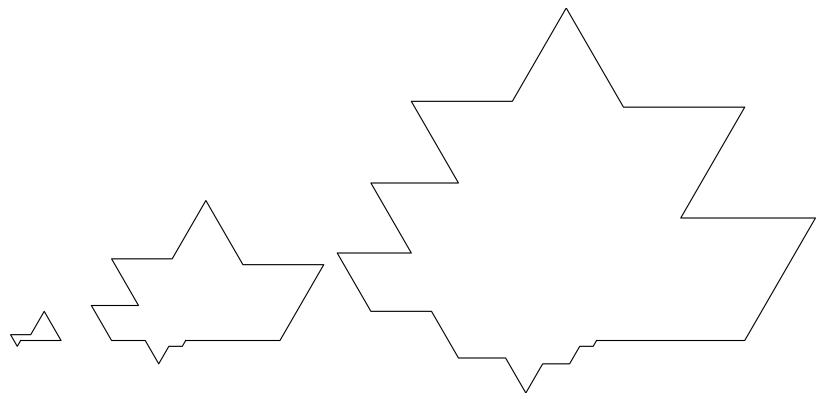
\includegraphics[width=4.5in]{4th_degree_area.png}
\captionof{figure}{Polyiamond sequence $\mathcal{P}^{(8,6)}_k$.}
\label{fig:4th_degree_area}
}} 

In terms of $n$, the area $A(\mathcal{P}^{(8,6)}_k) = 44k^4 + 252k^3 + 362k^2 + 190k + 31$ 
is also a polynomial of degree $4$ in $n$: $A(n) = \frac{11}{1024}n^4 + o(n^4)$.
The maximum area of a perfect $n$-polyiamond should not exceed $A(n) = \frac{1}{32}n^4 + o(n^4)$.

{\centering{
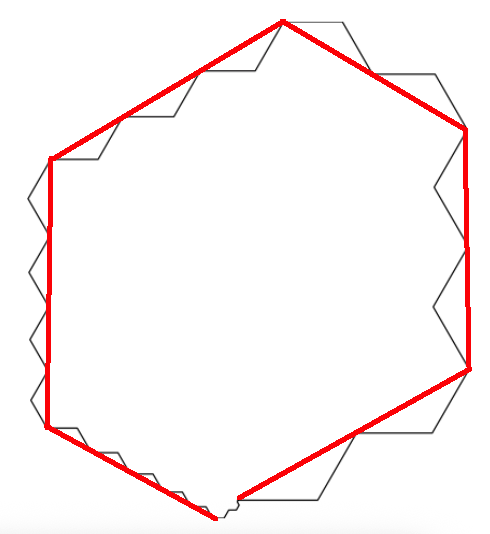
\includegraphics[width=2.5in]{polyiamond42.png}
\captionof{figure}{A $42$-sided perfect polyiamond approximating a hexagon; area $284674$.}
\label{fig:polyiamond42}
}} 


The estimate $\frac{1}{32}n^4 + o(n^4)$ for the maximum area of a perfect $n$-polyiamond
comes from {\em W. C. Yang and R. R. Meyer, Maximal and minimal polyiamonds, Technical Report, University of Wisconsin–Madison, 2002}, 
which states that the number of unit triangles within a polyiamond of perimeter $P$ cannot exceed 
the rounded integer
\[ \frac{p^2}{6} - \begin{cases} 0 & p \equiv 0 \pmod 6 \\ 1 & \text{else}\end{cases}. \]
For perfect polyiamonds, $p = n(n+1)/2$; and for large $n$ the perimeter $p$ participates in zig-zaging where the 
projection of each side to the reference hexagon is $\cos 30^{\circ} = \sqrt{3}/2$.






\end{document}